\section{固有振動モードの変動に関する方程式}

\begin{figure}[ht]
	\begin{center}
		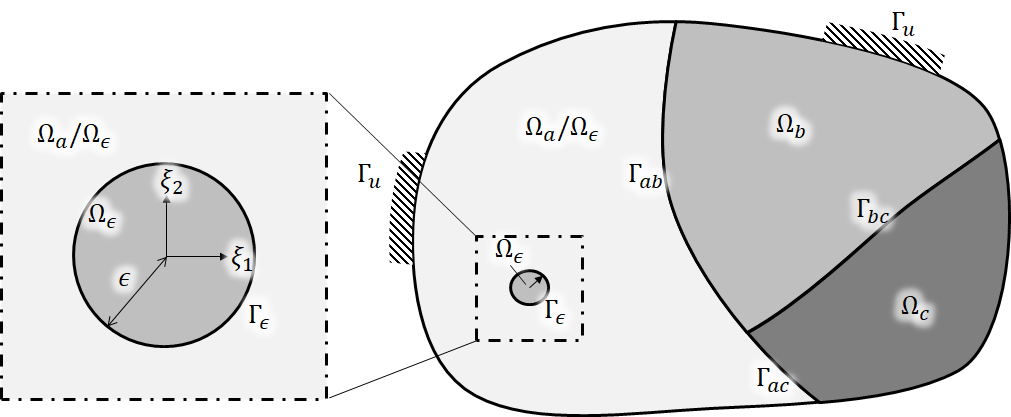
\includegraphics[width=13cm]{./figures/TD.png}
		\caption{Topological derivative}
		\label{fig:TD}
	\end{center}
\end{figure}

材料$a$で占められた領域$\Omega_a$中の微小な円領域$\Omega_\epsilon$に材料$b$が生成した際の,固有振動モード$\bm{u}^{\epsilon}$および固有値$\lambda^{\epsilon}$について考える.
ただし,これによって固有振動モードの次数の変化は起こらないと仮定する.
この時の支配方程式は以下のようになる.
\begin{align}
	&C_{ijkl}^{b}u_{k,lj}^{\epsilon}+\lambda^{\epsilon}\rho^{b} u_{i}^{\epsilon}=0&&\text{in}\hspace{0.3cm}\Omega_{\epsilon}
	\label{eq:govepmain}
	\\
	&C_{ijkl}^{a}u_{k,lj}^{\epsilon}+\lambda^{\epsilon}\rho^{a} u_{i}^{\epsilon}=0&&\text{in}\hspace{0.3cm}\Omega_{a}\backslash\Omega_{\epsilon}
	\label{eq:govepmain}
	\\
	&C_{ijkl}^{p}u_{k,lj}^{\epsilon}+\lambda^{\epsilon}\rho^{p} u_{i}^{\epsilon}=0&&\text{in}\hspace{0.3cm}\Omega_{p}\hspace{0.3cm}(p\neq a)
	\label{eq:govepmain}
	\\
	&u_{i}^{\epsilon b}=u_{i}^{\epsilon a} &&\text{on}\hspace{0.3cm}\Gamma_{\epsilon}
	\\
	&C_{ijkl}^{b}u_{k,l}^{\epsilon b}n_{j}^{b}+C_{ijkl}^{a}u_{k,l}^{\epsilon a}n_{j}^{a}=0 &&\text{on}\hspace{0.3cm}\Gamma_{\epsilon}
	\label{eq:govepbc}
	\\
	&u_{i}^{\epsilon p}=u_{i}^{\epsilon q} &&\text{on}\hspace{0.3cm}\Gamma_{pq}
	\\
	&C_{ijkl}^{p}u_{k,l}^{\epsilon p}n_{j}^{p}+C_{ijkl}^{q}u_{k,l}^{\epsilon q}n_{j}^{q}=0 &&\text{on}\hspace{0.3cm}\Gamma_{pq}
	\label{eq:govepbc}
	\\
	&\sum_{p=1,p\neq a}^{n}\int_{\Omega_p}(\rho^{p}u_{i}^{\epsilon}u_{i}^{\epsilon}) d\Omega
	+\int_{\Omega_a\backslash\Omega_{\epsilon}}(\rho^{a}u_{i}^{\epsilon}u_{i}^{\epsilon}) d\Omega
	+\int_{\Omega_{\epsilon}}(\rho^{b}u_{i}^{\epsilon}u_{i}^{\epsilon}) d\Omega=1
	\label{eq:govepnorm}
\end{align}

$\bm{u}^{\epsilon},\lambda^{\epsilon}$を,微小な材料$b$の領域が生成される前の固有ベクトルおよび固有値$\bm{u},\lambda$用いて展開すると,次式のようになる。
\begin{align}
	\bm{u}^{\epsilon}(\bm{x})=&\bm{u}(\bm{x})\chi_{R^2/\Omega}+\hat{\bm{u}}(\bm{x})
	\\
	\lambda^{\epsilon}=&\lambda+\hat{\lambda}
\end{align}
ここで,$\Omega_\epsilon$の中心座標を$\bm{x}_0$とし,$\bm{\xi}=\frac{\bm{x}-\bm{x}_0}{\epsilon}$を導入し,
$\hat{\bm{u}}(\bm{x})$を$\epsilon$に関して次式のように漸近展開する.
\begin{align}
	\hat{\bm{u}}(\bm{x})
	=&\{\hat{\bm{u}}^{(I-)}(\bm{x})+\epsilon\hat{\bm{u}}^{(I\hspace{-.1em}I-)}(\bm{x})\}\chi_{\Omega_\epsilon}
	+\{\hat{\bm{u}}^{(I+)}(\bm{x})+\epsilon\hat{\bm{u}}^{(I\hspace{-.2em}I+)}(\bm{x})\}\chi_{R^2\backslash\Omega_\epsilon}+O(\epsilon^2)
	\nonumber
	\\
	=&\{\hat{\bm{w}}^{(I-)}(\bm{\xi})+\epsilon\hat{\bm{w}}^{(I\hspace{-.1em}I-)}(\bm{\xi})\}\chi_{\Omega_\epsilon}
	+\{\hat{\bm{w}}^{(I+)}(\bm{\xi})+\epsilon\hat{\bm{w}}^{(I\hspace{-.2em}I+)}(\bm{\xi})\}\chi_{R^2\backslash\Omega_\epsilon}+O(\epsilon^2)
	\nonumber
	\\
	=&\{\hat{\bm{w}}^{(-)}(\bm{\xi})\}\chi_{\Omega_\epsilon}
	+\{\hat{\bm{w}}^{(+)}(\bm{\xi})\}\chi_{R^2\backslash\Omega_\epsilon}+O(\epsilon^2)
\end{align}
ただし,上付き添え字の+は微小領域の外側を-は内側を示している.
この時,$\hat{\bm{w}}(\bm{\xi})^{(\pm)}$は次式を満たす.
\begin{align}
	&C_{ijkl}^{b} \Bigl \{ \frac{1}{\epsilon^2}\frac{\partial^2 \hat{w}^{(-)}_{k}} {\partial \xi_l \partial \xi_j}(\bm{\xi})\Bigr \}
	+\bigl( \lambda+\hat{\lambda}\bigr) \rho^{b} 
	 \hat{w}_{i}^{(-)}(\bm{\xi})=0
	&&\text{in}\hspace{0.3cm}\Omega_{\epsilon}
	\label{eq:GovEpsIn}
	\\
	&C_{ijkl}^{a} \Bigl \{ \frac{\partial^2 u^{}_{k}} {\partial x_l \partial x_j}(\bm{x})
	+\frac{1}{\epsilon^2}\frac{\partial^2 \hat{w}^{(+)}_{k}} {\partial \xi_l \partial \xi_j}(\bm{\xi})\Bigr \}
	+\bigl( \lambda+\hat{\lambda}\bigr) \rho^{a}
	\bigl \{ u_{i}^{}(\bm{x})+\hat{w}_{i}^{(+)}(\bm{\xi})\bigr \}=0
	&&\text{in}\hspace{0.3cm}\Omega_{a}\backslash\Omega_{\epsilon}
	\label{eq:GovEpsOut}
	\\
	&\hat{w}_{i}^{(-)}(\bm{\xi})=u_{i}^{}(\bm{x})+\hat{w}_{i}^{(+)}(\bm{\xi})
	&&\text{on}\hspace{0.3cm}\Gamma_{\epsilon}
	\\
	&C_{ijkl}^{b} \Bigl \{ \frac{1}{\epsilon}\frac{\partial \hat{w}^{(-)}_{k}} {\partial \xi_l}(\bm{\xi}) n_{j}^{(-)} \Bigr \}
	+C_{ijkl}^{a} \Bigl \{ \frac{\partial u^{}_{k}} {\partial x_l}(\bm{x})n_{j}^{(+)}
	+\frac{1}{\epsilon}\frac{\partial \hat{w}^{(+)}_{k}} {\partial \xi_l}(\bm{\xi}) n_{j}^{(+)} \Bigr \}
	=0
	&&\text{on}\hspace{0.3cm}\Gamma_{\epsilon}
	\label{eq:GovEpsBC}
\end{align}
\begin{align}
	&\sum_{p=1,p\neq a}^{n}\int_{\Omega_p}\rho^{p}(u_{i}u_{i}+2u_{i}\hat{w}_{i}^{(+)}+\hat{w}_{i}^{(+)}\hat{w}_{i}^{(+)}) d\Omega
	\nonumber
	\\
	&\hspace{1.0cm}+\int_{\Omega_a\backslash\Omega_{\epsilon}}\rho^{a}(u_{i}u_{i}+2u_{i}\hat{w}_{i}^{(+)}+\hat{w}_{i}^{(+)}\hat{w}_{i}^{(+)}) d\Omega
	+\int_{\Omega_{\epsilon}}\rho^{b}(\hat{w}_{i}^{(-)}\hat{w}_{i}^{(-)}) d\Omega=1
	\label{eq:GovEpsNorm}
\end{align}

式\eqref{eq:GovEpsOut}から式\eqref{eq:Gov}を引き,整理することで,以下のようになる.
\begin{align}
	&C_{ijkl}^{b} \hat{w}^{(-)}_{k,lj}(\bm{\xi})
	+\epsilon^2\Bigl\{(\lambda+\hat{\lambda})\rho^{b} \hat{w}_{i}^{(-)}(\bm{\xi})\Bigr\}=0
	&&\text{in}\hspace{0.3cm}\Omega_{\epsilon}
	\label{eq:GovDisturIn}
	\\
	&C_{ijkl}^{a}\hat{w}^{(+)}_{k,lj}(\bm{\xi})
	+\epsilon^2\Bigl \{\lambda\rho^{a} \hat{w}_{i}^{(+)}(\bm{\xi})
	+\hat{\lambda}\rho^{a} \Bigl(u_{i}^{}(\bm{x})+\hat{w}_{i}^{(+)}(\bm{\xi}) \Bigr) \Bigr \}=0
	&&\text{in}\hspace{0.3cm}\Omega_{a}\backslash\Omega_{\epsilon}
	\label{eq:GovDisturOut}
	\\
	&\hat{w}_{i}^{(-)}(\bm{\xi})-\hat{w}_{i}^{(+)}(\bm{\xi})=u_{i}(\bm{x})=u_{i}(\bm{x_0})+\epsilon \xi_j u_{i,j}(\bm{x_0})+O(\epsilon^2)
	&&\text{on}\hspace{0.3cm}\Gamma_{\epsilon}
	\label{eq:GovDisturUBC}
	\\
	&C_{ijkl}^{b}\hat{w}_{k,l}^{(-)}(\bm{\xi})n_{j}^{(-)}
	-C_{ijkl}^{a}\hat{w}_{k,l}^{(+)}(\bm{\xi})n_{j}^{(-)}
	=\epsilon C_{ijkl}^{a}u_{k,l}(\bm{x_0})n_{j}^{(-)}+O(\epsilon^2)
	&&\text{on}\hspace{0.3cm}\Gamma_{\epsilon}
	\label{eq:GovDisturSBC}
\end{align}
\begin{align}
	\sum_{p=1}^{n}\int_{\Omega_p}\rho^{p}(2u_{i}\hat{w}_{i}^{(+)}+\hat{w}_{i}^{(+)}\hat{w}_{i}^{(+)}) d\Omega
	+\int_{\Omega_{\epsilon}}\{\rho^{b}\hat{w}_{i}^{(-)}\hat{w}_{i}^{(-)}-\rho^{a}u_{i}u_{i}\} d\Omega=0
	\label{eq:GovDisturNorm}
%	\\
%	\hat{w}_{i}^{(+)}(\bm{\xi})\rightarrow 0 \hspace{0.3cm} (|\bm{\xi}|\rightarrow \infty)
%	\hspace{4.5cm}
%	\label{eq:GovDisturInftyBC}
\end{align}

$\epsilon$の0次の項を整理すると
\begin{align}
	C_{ijkl}^{b} \hat{w}^{(I-)}_{k,lj}(\bm{\xi})=0
	\hspace{1.7cm}\text{in}\hspace{0.3cm}\Omega_{\epsilon}
	\label{eq:GovDisturIn1}
	\\
	C_{ijkl}^{a} \hat{w}^{(I+)}_{k,lj}(\bm{\xi})=0
	\hspace{1.2cm}\text{in}\hspace{0.3cm}\Omega\backslash\Omega_{\epsilon}
	\label{eq:GovDisturOut1}
	\\
	\hat{w}_{i}^{(I-)}(\bm{\xi})-\hat{w}_{i}^{(I+)}(\bm{\xi})=u_{i}(\bm{x_0})
	\hspace{0.7cm}\text{on}\hspace{0.3cm}\Gamma_{\epsilon}
	\label{eq:GovDisturUBC1}
	\\
	C_{ijkl}^{b}\hat{w}_{k,l}^{(I-)}(\bm{\xi})n_{j}^{(-)}
	-C_{ijkl}^{a}\hat{w}_{k,l}^{(I+)}(\bm{\xi})n_{j}^{(-)}=0
	\hspace{1.5cm}\text{on}\hspace{0.3cm}\Gamma_{\epsilon}
	\label{eq:GovDisturSBC1}
%	\\
%	\hat{w}_{i}^{(I+)}(\bm{\xi})\rightarrow 0\hspace{0.3cm} (|\bm{\xi}|\rightarrow \infty)
%	\hspace{2.0cm}
%	\label{eq:GovDisturInftyBC1}
\end{align}

$\epsilon$の1次の項を整理すると
\begin{align}
	C_{ijkl}^{b} \hat{w}^{(I\hspace{-.15em}I-)}_{k,lj}(\bm{\xi})=0
	\hspace{2.5cm}
	\text{in}\hspace{0.3cm}\Omega_{\epsilon}
	\label{eq:GovDisturIn2}
	\\
	C_{ijkl}^{a} \hat{w}^{(I\hspace{-.15em}I+)}_{k,lj}(\bm{\xi})=0
	\hspace{2.0cm}
	\text{in}\hspace{0.3cm}\Omega\backslash\Omega_{\epsilon}
	\label{eq:GovDisturOut2}
	\\
	\hat{w}_{i}^{(I\hspace{-.15em}I-)}(\bm{\xi})
	-\hat{w}_{i}^{(I\hspace{-.15em}I+)}(\bm{\xi})= \xi_j u_{i,j}(\bm{x_0})
	\hspace{2.0cm}
	\nonumber
	\\
	\equiv u_{i}^{(I\hspace{-.15em}I)}
	\hspace{1.9cm}\text{on}\hspace{0.3cm}\Gamma_{\epsilon}
	\label{eq:GovDisturUBC2}
	\\
	C_{ijkl}^{b}\hat{w}_{k,l}^{(I\hspace{-.15em}I-)}(\bm{\xi})n_{j}^{(-)}
	-C_{ijkl}^{a}\hat{w}_{k,l}^{(I\hspace{-.15em}I+)}(\bm{\xi})n_{j}^{(-)}
	=C_{ijkl}^{a} u_{k,l}^{}(\bm{x_0})n_{j}^{(-)}
	\hspace{1.0cm}
	\nonumber
	\\
	\equiv t_{i}^{(I\hspace{-.15em}I)}
	\hspace{2.0cm}\text{on}\hspace{0.3cm}\Gamma_{\epsilon}
	\label{eq:GovDisturSBC2}
%	\\
%	\hat{w}_{i}^{(I\hspace{-.15em}I+)}(\bm{\xi})\rightarrow 0 \hspace{0.3cm} (|\bm{\xi}|\rightarrow \infty)
%	\hspace{3.0cm}
%	\label{eq:GovDisturInftyBC2}
\end{align}
以上から,$\hat{\bm{w}}^{(I-)}$,$\hat{\bm{w}}^{(I+)}$,$\hat{\bm{w}}^{(I\hspace{-.15em}I-)}$,$\hat{\bm{w}}^{(I\hspace{-.15em}I+)}$は,それぞれ平衡方程式に従うことが分かる.

\newpage
